\subsection{I sistemi di riferimento inerziali}
Come ogni ambito della fisica la descrizione matematica dei sistemi di riferimento necessita di una serie di osservazioni sperimentali da utilizzare assiomaticamente.\\

Il primo fatto sperimentale che viene assunto è che lo spazio sia tridimensionale, isotropo e omogeneo, ossia che non esistano rispettivamente direzioni e punti privilegiati ma che siano tutti equivalenti. Inoltre si assume che lo spazio rispetti la 
geometria euclidea mentre il tempo sia ad una sola dimensione ed anch'esso isotropo ed omogeneo.\\
Sulla base di queste assunzioni si può quindi scegliere un punto dello spazio-tempo come 
vettore nullo di uno spazio vettoriale 
$\mathbb{R}\times\mathbb{R}^3$, quindi da questo vengono scelte tre direzioni spaziali arbitrarie lungo le quali sono orientati tre assi cartesiani, identificabili con la base di $\mathbb{R}^3$. 
Inoltre dall'istante corrispondente al punto spazio-temporale precedentemente scelto si inizia a misurare il tempo. Si osservi che tali scelte sono arbitrarie poiché spazio e tempo sono assunti essere isotropi ed omogenei.\\

Per poter formulare delle leggi che descrivano la realtà risulta necessario assumere che esistano una serie di sistemi di riferimento, detti inerziali, in cui tali leggi sono valide indipendentemente dal sistema in cui sono descritte. Questi sistemi sono sperimentalmente caratterizzati dalla proprietà di essere reciprocamente in moto rettilineo uniforme, ossia che il moto dell'origine di un sistema visto in un qualsiasi altro sistema di riferimento inerziale deve essere nella forma: 
\begin{equation}
	\vec x(t)=\vec x_0+\vec vt \qquad \vec x_0,\vec v\in \mathbb{R}^3, \ t\in\mathbb{R},
\end{equation}
dove $\vec x$ è rappresnta un punto nello spazio, $t$ un istante di tempo e $\vec v$ la velocità reciproca dei due sistemi di riferimento che risulta identicamente costante.\\
Una volta identificati questi particolari sistemi  si può enunciare il principio di relatività: \emph{in ogni sistema di riferimento inerziale tutte le leggi della fisica sono identiche}.\\

\subsection{Trasformazioni di sistemi di riferimento inerziali}
Si vuole ora studiare quali siano le più generiche trasformazioni che consentono di ottenere la descrizione di un moto in un sistema di riferimento inerziale $K'$ conoscendo la descrizione di tale moto in un primo riferimento inerziale $K$. In questo modo la generica trasformazione da $K$ a $K'$ sarà un'applicazione $f:\mathbb{R}\times \mathbb{R}^3\rightarrow\mathbb{R}\times \mathbb{R}^3$ invertibile; quest'ultima propreità è necessaria poiché come deve essere possibile passare da $K$ a $K'$ deve essere possibile fare il contrario.\\
Per poter caratterizzare le proprietà di tale applicazione è ora necessario tradurre matematicamente la richiesta imposta dal principio di relatività. Si osservi che per tale principio e per la definizione di sistema inerziale è necessario che in seguito ad una trasformazione tutti i sistemi inerziali restino tali, in altre parole è necessario che ogni retta spaziotemporale venga trasformata in un'altra retta spazitemporale, poiché rettilineo ed uniforme è il moto caratteristico di questi sistemi di riferimento. Questa condizione soddisfa le ipotesi di un teorema$^{\cite{LostThmOfGeometry}}$ di geometria che consente di identificare la famiglia di queste trasformazioni.

\begin{thm}
Sia $f:\mathbb{R}^n\rightarrow\mathbb{R}^n\ (n>1)$ una funzione biettiva che trasforma rette in altre rette. Allora $f$ è una trasformazione affine. 
\label{thm:LinGenMain}
\end{thm}
Per procedere alla dimostrazione di questo teorema è utile iniziare dimostrandone un caso particolare, ossia il caso $n=2$. Per questo caso particolare è però necessario dimostrare in primo luogo un risultato preliminare:
\begin{prop}
	Sia $\varphi:\mathbb{R}\rightarrow\mathbb{R}$ un automorfismo di campo, ossia tale che se presi $x,y\in \mathbb{R}$ valgano $\varphi(x+y)=\varphi(x)+\varphi(y)$ e $\varphi(xy)=\varphi(x)\varphi(y)$.
	Allora $\varphi=\text{id}$.
\end{prop}	
\begin{proof}
	Si osservi che $\varphi(1)=1$ infatti se $x\neq0$ allora $\varphi(x)=\varphi(1\cdot x)=\varphi(1)\varphi(x)$. Inoltre $\varphi(0)=0$, infatti $\forall x\in\mathbb{R}$ vale $\varphi(0\cdot x)=\varphi(0)\varphi(x)=\varphi(0)$, questa equazione implica $\varphi(0)(\varphi(x)-1)=0$ che risulta soddisfatta per ogni $x$ solo se $\varphi(0)$ è identicamente nullo. Queste proprietà garantiscono che $\varphi(-1)=-1$, infatti $\varphi(1-1)=\varphi(1)+\varphi(-1)=\varphi(0)=0$.\\
	Si prenda ora $n\in\mathbb{N}$, $n$ è esprimibile come somma ripetuta $n$ volte dell'unità, in questo modo si ottiene che:
	\begin{equation*}
		\varphi(n)=\varphi(1+1+...+1)=n\varphi(1)=n.
	\end{equation*}
	Dalle proprietà precedentemente descritte è immediato che $\varphi(n)=n$ valga per ogni numero intero poiché $\varphi(-n)=-1\varphi(n)=-n$.\\
	Si consideri adesso $q\in \mathbb{Q}$ allora $\varphi(q)=q$. Infatti, se $x,y\in\mathbb{R}$ tali che $xy=1$, per quanto già detto, $\varphi(xy)=\varphi(x)\varphi(y)=1$ e quindi $\varphi(\frac{1}{x})=\frac{1}{\varphi(x)}$. Poiché ogni numero razionale è esprimibile come rapporto di numeri interi si ha che pure questi sono conservati da $\varphi$.\\
	Siano $x,y\in \mathbb{R}$ con $x<y$, allora $\exists z\in\mathbb{R}$ tale che $z\neq0$ e $y-x=z^2$. Utilizzando le proprietà supposte per ipotesi si ha quindi che:
	\begin{equation*}
		\varphi(y)-\varphi(x)=\varphi(y-x)=\varphi(z^2)=\varphi(z)^2>0.
	\end{equation*}
	Questo implica che $\varphi$ conservi l'ordinamento di $\mathbb{R}$.\\
	Sia ora $x\in\mathbb{R}$, poiché $\varphi(x)\in\mathbb{R}$ e $\mathbb{Q}$ è denso in $\mathbb{R}$ allora se $x\neq\varphi(x)$ deve esistere un $q\in\mathbb{Q}$ compreso tra $\varphi(x)$ e $x$. Si supponga $\varphi(x)>x$, in maniera del tutto analoga si può procedere supponendo $\varphi(x)<x$, allora $\varphi(x)> q> x$, poiché $\varphi$ conserva l'ordinamento si ha $\varphi(q)>\varphi(x)$, al contempo $q=\varphi(q)$. Da questo ragionamento si deduce che $\varphi(x)> q>\varphi(x)$, ossia che $q=\varphi(q)=\varphi(x)$. Questo risultato è però in contraddizione con la proprietà di densità per cui si conclude che $\varphi=\text{id}$.
\end{proof}
\begin{thm}
	Sia $f:\mathbb{R}^2\rightarrow\mathbb{R}^2$ una funzione biettiva che trasforma rette in altre rette. Allora $f$ è una trasformazione affine. 
	\label{thm:LinGen2}
\end{thm}
\begin{proof}
    Sia $A:\mathbb{R}^2\rightarrow\mathbb{R}^2$ una trasformazione affine invertibile tale che $(A\circ f)(0,0)=(0,0),\ (A\circ f)(1,0)=(1,0)$ e $(A\circ f)(0,1)=(0,1)$. Si osservi che anche $A\circ f$ trasforma rette in rette poiché la trasformazione affine può agire su una retta solamente ruotandola e traslandola. Si dirà $(A\circ f)(x)=g(x)$.\\
	
	Si considerino i punti $x,y$ e $(0,0)$ non giacenti sulla stessa retta nel piano $\mathbb{R}^2$. Si prendano due rette passanti rispettivamente per l'origine e $x$ e l'origine e $y$ e le rispettive rette parallele passanti per $y$ nel primo caso e $x$ nel secondo, come mostrato in Figura \ref{Fig:PianoLinGen}, queste ultime due rette si intersecheranno nel punto $x+y$, formando quindi un parallelogrammo.\\
	\begin{figure}[h!]
		\centering
		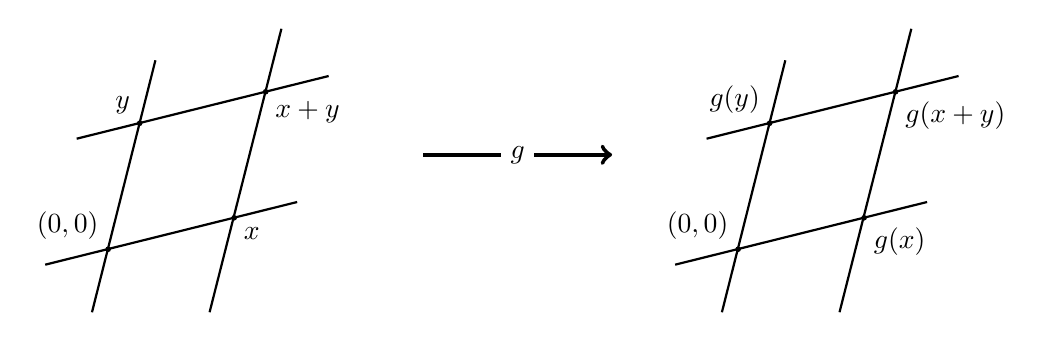
\begin{tikzpicture}[scale=0.8]
		\filldraw[black] (0,0) circle (1pt) node[anchor=south east]{$(0,0)$};
		\filldraw[black] (.5,2) circle (1pt) node[anchor=south east]{$y$};
		\filldraw[black] (2,.5) circle (1pt) node[anchor=north west]{$x$};
		\filldraw[black] (2.5,2.5) circle (1pt) node[anchor=north west]{$x+y$};

		\draw[black, thick] (-1,-0.245) -- (3,0.75);
		\draw[black, thick] (-.5,1.755) -- (3.5,2.75);
		\draw[black, thick] (-0.257,-1) -- (0.75,3);
		\draw[black, thick] (1.61,-1) -- (2.75,3.5);

		\filldraw[black] (0+10,0) circle (1pt) node[anchor=south east]{$(0,0)$};
		\filldraw[black] (.5+10,2) circle (1pt) node[anchor=south east]{$g(y)$};
		\filldraw[black] (2+10,.5) circle (1pt) node[anchor=north west]{$g(x)$};
		\filldraw[black] (2.5+10,2.5) circle (1pt) node[anchor=north west]{$g(x+y)$};

		\draw[black, thick] (-1+10,-0.245) -- (3+10,0.75);
		\draw[black, thick] (-.5+10,1.755) -- (3.5+10,2.75);
		\draw[black, thick] (-0.257+10,-1) -- (0.75+10,3);
		\draw[black, thick] (1.61+10,-1) -- (2.75+10,3.5);

		\draw[black, ultra thick,->] (5,1.5) -- (8,1.5);
		\node[fill=white] at (6.5,1.5) {$g$};
		
	\end{tikzpicture}
	\caption{Rappresentazione grafica di come agisce la funzione $g$ nel piano}
	\label{Fig:PianoLinGen}
	\end{figure}
	Per ipotesi queste quattro rette verranno mappate in altre quattro rette da $g$ e poiché questa funzione è biettiva le immagini di rette parallele saranno a loro volta parallele, altrimenti nel punto di incidenza si perderebbe l'iniettività, mentre i punti di incidenza potranno essere mappati solamente in altri punti di incidenza poiché questi appartenendo al dominio di due rette ognuno dovranno, per biettività, appartenere ad entrambe le immagini delle due rette nel codominio. Questo sta a significare che le quattro rette così ottenute formeranno un novo parallelogrammo di vertici $g(x),\ g(y),\ g(x+y)$ e $(0,0)$, poiché per costruzione $g(0,0)=(0,0)$. La regola del parallelogramma garantisce quindi che $g(x)+g(y)=g(x+y)$.\\
	Se invece i punti $x,y$ e $(0,0)$ giacciono sulla stessa retta è sufficiente prendere un punto $z\in \mathbb{R}^2$ che non giaccia sulla medesima retta dei punti precedenti. Si può quindi utilizzare quanto dimostrato nel caso precedente per ottenere:
	\begin{equation*}
		g(x+y+z)=g(x+y)+g(z)= g(x)+g(y+z)=g(x)+g(y)+g(z)
	\end{equation*}
	da cui segue che $g(x+y)=g(x)+g(y)$ anche in questo caso.\\

    Poiché per ipotesi $g$ conserva le rette del piano e per costruzione mappa l'origine nell'origine e i punti $(0,1)$ e $(1,0)$ in se stessi allora $g$ deve trasformare gli assi $x$ e $y$ in se stessi. Si possono quindi considerare due applicazioni $\alpha,\beta:\mathbb{R} \rightarrow\mathbb{R} $ tali che $g(x,y)=(\alpha(x),\beta(y))$ con  $x,y\in\mathbb{R}$. Si osservi che per quanto dimostrato fino ad ora $f(1,1)=f(1,0)+f(0,1)=(1,0)+(0,1)=(1,1)$, analogamente a come si è detto per gli assi $x$ e $y$ anche la bisettrice del primo quadrante è quindi mappata in se stessa per cui per ogni $x\in\mathbb{R}$ $\alpha(x)=\beta(x)$. Si proseguirà quindi studiando solo una di queste due funzioni poiché quanto si dirà per una è valido anche per l'altra.\\

	Siano $a,b\in\mathbb{R}$ e si consideri una retta passante per l'origine.
	\begin{equation*}
		L=\{ (x,y)\in\mathbb{R}^2 \text{ tale che } y=ax\  \}
	\end{equation*}
    Il punto $(1,a)\in L$ e poiché $g(1,a)=(1,\alpha(a))$ si ottiene che $L$ è mappata in una nuova retta passante per l'origine con coefficiente angolare $\alpha(a)$.
	\begin{equation*}
		g(L)=\{ (x,y)\in\mathbb{R}^2 \text{ tale che } y=\alpha(a)x\}
	\end{equation*} 
	Pure $(b,ab)\in L$ e quindi $(\alpha(b),\alpha(ab))\in g(L)$, ricordando però che $g(L)$ è una retta passante per l'origine con coefficiente angolare $\alpha(a)$ si deduce che dovrà sussistere la seguente relazione: $\alpha(ab)=\alpha(a)\alpha(b)$.\\

	Si è quindi dimostrato che per $\alpha$ e $\beta$ valgono le seguenti relazioni per ogni $x,y\in\mathbb{R}$:
	\begin{flalign*}
		&&\alpha(x+y)=\alpha(x)+\alpha(y)\qquad \alpha(xy)=\alpha(x)\alpha(y)&&\\
		&&\beta(x+y)=\beta(x)+\beta(y)\qquad \beta(xy)=\beta(x)\beta(y).&&
	\end{flalign*}
	Queste relazioni implicano che $\alpha$ e $\beta$ siano due automorfismi di campo di $\mathbb{R}$ e per la proposizione inizialmente dimostrata risultano entrambi l'identità, di conseguenza pure $g=A\circ f=\text{id}$. Infine è sufficiente appllicare a $g$ la trasformazione inversa di $A$ così da avere $A^{-1}\circ A\circ f=A^{-1}=f$, per cui si è dimostrato che $f$ deve essere affine.
\end{proof}

Si procederà ora generalizzando questo teorema con la dimostrazione del teorema \ref{thm:LinGenMain}.

\begin{proof}[Dimostrazione teorema \ref{thm:LinGenMain} $(n>2)$]
	Si consideri la traslazione $T:\mathbb{R}^n \rightarrow\mathbb{R}^n$ tale che $(T\circ f)(0)=0$, si dirà $(T\circ f)(x)=g(x)$.\\
	Siano $x,y\in\mathbb{R}^n$ e $\pi$ un piano tale che $x,y\in\pi$. Si prendano due rette $r_1,r_2\in\pi$ e incidenti in $O$, e un punto $P\in\pi$. Se si considerano altre due rette $r_3$ e $r_4$ passanti per $P$ e tali che $r_3$ sia parallela a $r_1$ e $r_4$ lo sia per $r_2$, così che $r_3$ intersecherà $r_2$ in un punto $P_2$ e analogamente $r_4$ intersecherà $r_1$ in un punto $P_1$, è possibile costruire un parallelogrammo con vertice $P$ e lati giacenti sulle rette considerate.
	\begin{figure}[h!]
		\centering
		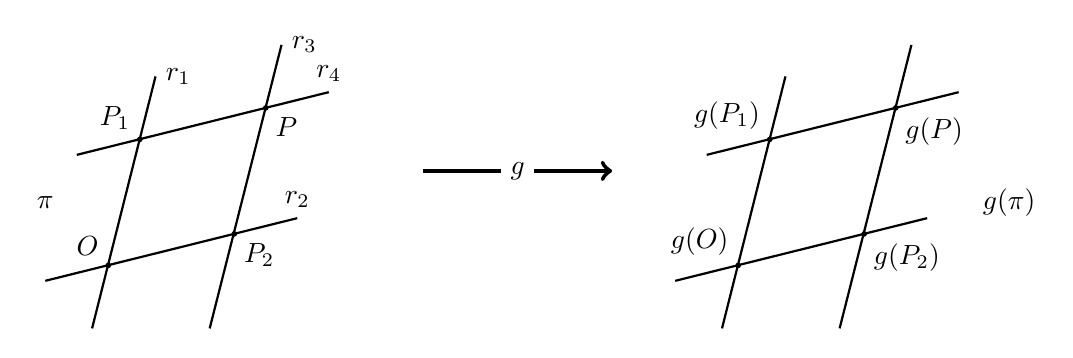
\begin{tikzpicture}[scale=0.8]
		\filldraw[black] (0,0) circle (1pt) node[anchor=south east]{$O$};
		\filldraw[black] (.5,2) circle (1pt) node[anchor=south east]{$P_1$};
		\filldraw[black] (2,.5) circle (1pt) node[anchor=north west]{$P_2$};
		\filldraw[black] (2.5,2.5) circle (1pt) node[anchor=north west]{$P$};

		\draw[black, thick] (-1,-0.245) -- (3,0.75) node[anchor=south]{$r_2$};
		\draw[black, thick] (-.5,1.755) -- (3.5,2.75) node[anchor=south]{$r_4$};
		\draw[black, thick] (-0.257,-1) -- (0.75,3) node[anchor=west]{$r_1$};
		\draw[black, thick] (1.61,-1) -- (2.75,3.5) node[anchor=west]{$r_3$};

		\filldraw[black] (0+10,0) circle (1pt) node[anchor=south east]{$g(O)$};
		\filldraw[black] (.5+10,2) circle (1pt) node[anchor=south east]{$g(P_1)$};
		\filldraw[black] (2+10,.5) circle (1pt) node[anchor=north west]{$g(P_2)$};
		\filldraw[black] (2.5+10,2.5) circle (1pt) node[anchor=north west]{$g(P)$};

		\draw[black, thick] (-1+10,-0.245) -- (3+10,0.75) ;
		\draw[black, thick] (-.5+10,1.755) -- (3.5+10,2.75) ;
		\draw[black, thick] (-0.257+10,-1) -- (0.75+10,3) ; 
		\draw[black, thick] (1.61+10,-1) -- (2.75+10,3.5) ;

		\draw[black, ultra thick,->] (5,1.5) -- (8,1.5);
		\node[fill=white] at (6.5,1.5) {$g$};
		\node[fill=white] at (-1,1) {$\pi$};
		\node[fill=white] at (14.3,1) {$g(\pi)$};
		
	\end{tikzpicture}
	\caption{Rappresentazione grafica di come agisce la funzione $g$ nel piano}
	\label{Fig:PianoLinGen2}
\end{figure}
	 Poiché $g$ è biettiva e trasforma rette in rette allora, come si è già visto per dimostrare il teorema \ref{thm:LinGen2}, questo parallelogrammo deve essere trasformato in un nuovo parallelogrammo con i lati giacenti sulle immagini delle precedenti rette e con i vertici dati dalle immagini dei vertici del precedente parallelogrammo. Detto $\pi'$ il piano contente le immagini di $r_1$ e $r_2$ allora per costruzione del parallelogrammo si avrà che $g(P)\in \pi'$ e poiché $P\in\pi$ è arbitrario si deduce che ogni punto di $\pi$ è mappato in $\pi'$ ossia $g$ trasforma piani in altri piani.\\

	Si consideri ora un'applicazione lineare invertibile $L$ tale che $(L\circ g)(\pi)=\pi$, in questo modo $L\circ g\big|_{\pi}:\mathbb{R} ^2\rightarrow\mathbb{R} ^2$ è biettiva e trasforma rette in rette, per il teorema \ref{thm:LinGen2} allora questa è un'applicazione affine, nella fattispecie poiché $g(0)=0$ per costruzione e $L$ è lineare allora $(L\circ g)(0)=0$, per cui $L\circ g$ è lineare. Risulta a questo punto sufficiente far uso dell'inversa di $L$ per ottenere:
	\begin{equation*}
		g(\alpha x+\beta y)=L^{-1}((L\circ g)(\alpha x+\beta y))=L^{-1}(\alpha (L\circ g)(x)+\beta (L\circ g)(y))=\alpha g(x)+ \beta g(y) \quad \alpha,\beta\in\mathbb{R},
	\end{equation*}
	poiché la scelta di $x$ e $y$ fatta prima di determinare il piano $\pi$ è arbitraria segue che $g$ è lineare e considerando $f=T^{-1}\circ g$ allora si ha che $f$ deve essere affine.
\end{proof}

Così facendo si conclude che ogni trasformazione di un sistema di riferimento inerziale in un altro debba essere necessariamente una trasformazione affine di qualche sorta. Ulteriori osservazioni sperimentali consentiranno di identificare famiglie più ristrette di queste trasformazioni.